\documentclass[12pt]{article}
\usepackage{sbc/template}
\usepackage{amssymb,array,color,enumitem,graphicx,listings,mathtools,url}
\usepackage[brazil]{babel}
\usepackage[utf8]{inputenc}

\DeclarePairedDelimiter\ceil{\lceil}{\rceil}
\DeclarePairedDelimiter\floor{\lfloor}{\rfloor}
\DeclareMathOperator\concat{\lvert\rvert}
\newcommand\Keccak{\textsc{Keccak}}

\definecolor{codegreen}{rgb}{0,0.6,0}
\definecolor{codegray}{rgb}{0.5,0.5,0.5}
\definecolor{codepurple}{rgb}{0.58,0,0.82}
\definecolor{backcolour}{rgb}{0.95,0.95,0.92}

\lstdefinestyle{mystyle}{
    commentstyle=\color{codegreen},
    keywordstyle=\color{blue},
    numberstyle=\tiny\color{codegray},
    stringstyle=\color{codepurple},
    basicstyle=\footnotesize\ttfamily,
    breaklines=true,
    numbers=left,
    showstringspaces=false,
    extendedchars=true,
    inputencoding=utf8,
    literate={ç}{{\c{c}}}1 {ã}{{\~a}}1 {ó}{{\'o}}1
}
\lstset{style=mystyle}

\sloppy

\title{Função de Hash Criptográfica SHA-3}

\author{Ranieri Althoff}

\address{Universidade Federal de Santa Catarina\\
Departamento de Informática e Estatística\\
Segurança em Computação}

\begin{document}

\maketitle

\section{Introdução}\label{sec:firstpage}

Uma função \textit{hash} é uma função que aceita um bloco de dados de tamanho
variável como entrada e produz um valor de tamanho fixo como saída, chamado de
valor de \textit{hash}. Esta função tem a forma:
\begin{center}
    $h = H(M)$
\end{center}

Onde:
\begin{itemize}
	\item h é o valor hash de tamanho fixo gerado pela função hash.
	\item H é função hash que gerou o valor h.
	\item M é o valor de entrada de tamanho variável.
\end{itemize}

Espera-se que uma função \textit{hash} produza valores $h$ que são
uniformemente distribuídos no contra-domínio e que são aparentemente
aleatórios, ou seja, a mudança de apenas um \textit{bit} em $M$ causará uma
mudança do valor $h$. Por esta característica, as funções \textit{hash} são
muito utilizadas para verificar se um determinado bloco de dados foi
indevidamente alterado.

As funções \textit{hash} apropriadas para o uso em segurança de computadores
são chamadas de ``função \textit{hash} criptográfica''. Este tipo de função
\textit{hash} é implementada por um algoritmo que torna inviável
computacionalmente encontrar:
\begin{itemize}
    \item um valor $M$ dado um determinado valor $h$:
        $M | H(M) = h$
    \item dois valores $M_1$ e $M_2$ que resultem no mesmo valor:
        $(M_1, M_2) | H(M_1) = H(M_2)$
\end{itemize}

Os principais casos de uso de funções \textit{hash} criptográficas são:
\begin{itemize}
    \item Autenticação de Mensagens: é um serviço de segurança onde é possível
        verificar que uma mensagem não foi alterada durante sua transmissão e
        que é proveniente do devido remetente.
    \item Assinatura Digital: é um serviço de segurança que permite a uma
        entidade assinar digitalmente um documento ou mensagem.
    \item Arquivo de Senhas de Uma Via: é uma forma de armazenar senhas usando
        o valor \textit{hash} da senha, permitindo sua posterior verificação
        sem a necessidade de armazenar a senha em claro, cifrá-la ou
        decifrá-la.
    \item Detecção de Perpetração ou Infeção de Sistemas: é um serviço de
        segurança em que é possível determinar se arquivos de um sistema foram
        alterados por terceiros sem a autorização dos usuários do sistema.
\end{itemize}

\subsection{Propriedades}

Como observado na seção anterior, uma função \textit{hash} criptográfica
precisa ter certas propriedades para permitir seu uso em segurança de
computadores. Nas seções a seguir estão destacadas algumas dessas propriedades.

Antes, define-se dois termos usados a seguir:
\begin{itemize}
    \item Pré-Imagem: um valor $M$ do domínio de uma função \textit{hash} dada
        pela fórmula $h = H(M)$ é denominado de “pré-imagem” do valor $h$.
    \item Colisão: para cada valor $h$ de tamanho $n$ \textit{bits} existe
        necessariamente mais de uma pré-imagem correspondente de tamanho $m$
        \textit{bits} se $m > n$, ou seja, existe uma ``colisão''.
\end{itemize}

O número de pré-imagens de $m$ \textit{bits} para cada valor $h$ de $n$
\textit{bits} é calculado pela formula $2^{m/n}$. Se permitimos um tamanho em
\textit{bits} arbitrariamente longo para as pré-imagens, isto aumentará ainda
mais a probabilidade de colisão durante o uso de uma função \textit{hash}.
Entretanto, os riscos de segurança são minimizados se a função de \textit{hash}
criptográfica oferecer as propriedades descritas nas próximas seções.

\subsubsection{Resistente a Pré-Imagem}

Uma função \textit{hash} criptográfica é resistente a pré-imagem quando esta é
uma função de uma via. Ou seja, embora seja computacionalmente fácil gerar um
valor $h$ a partir de uma pré-imagem $M$ usando a função de \textit{hash}, é
computacionalmente inviável gerar uma pré-imagem a partir do valor $h$.

Se uma função \textit{hash} não for resistente à pré-imagem, é possível atacar
uma mensagem autenticada $M_1$ para descobrir o valor secreto $S$ usado na
mensagem, permitindo assim ao perpetrante enviar uma outra mensagem $M_2$ ao
destinatário no lugar do remetente sem que o destinatário perceba a violação da
comunicação. O ataque ocorre da seguinte forma:
\begin{itemize}
    \item O perpetrante tem conhecimento do algoritmo de \textit{hash} usado na
        comunicação entre as partes.
    \item Ao escutar a comunicação, o perpetrante descobre qual é a mensagem
        $M$ e o valor de \textit{hash} $h$.
    \item Visto que a inversão da função de \textit{hash} é computacionalmente
        fácil, o perpetrante calcula $H^{-1}(h)$.
    \item Como $H^{-1}(h) = S || M$, o perpetrante descobre $S$.
\end{itemize}

Desta forma, o perpetrante pode utilizar a chave secreta $S$ no envio de uma
mensagem $M_2$ para o destinatário sem que este perceba a violação.

\subsubsection{Resistente a Segunda Pré-Imagem}

Uma função \textit{hash} criptográfica é resistente a segunda pré-imagem
quando esta função torna inviável computacionalmente encontrar uma pré-imagem
alternativa que gera o mesmo valor \textit{h} da primeira pré-imagem.

Se uma função de \textit{hash} não for resistente a segunda pré-imagem, um
perpetrante conseguirá substituir uma mensagem que utiliza um determinado valor
de \textit{hash}, mesmo que a função de \textit{hash} seja de uma via, ou seja,
resistente a pré-imagem.

\subsubsection{Resistente a Colisão}

Uma função \textit{hash} criptográfica é resistente a colisão quando esta
tornar inviável computacionalmente encontrar duas pré-imagens quaisquer que
possuam o mesmo valor de \textit{hash}. Neste caso, diferentemente da
resistência a segunda pré-imagem, não é dado uma pré-imagem inicial para a qual
precisa se achar uma segunda pré-imagem, mas é suficiente encontrar duas
pré-imagens quaisquer tal que $H(M_1) = H(M_2)$.

Quando uma função \textit{hash} é resistente a colisão, está é consequente
resistente a segunda pré-imagem. Porém, nem sem sempre uma função resistente a
segunda pré-imagem será resistente a colisão. Por isto, diz-se que uma função
\textit{hash} resistente a colisão é uma função de \textit{hash} forte.

Se uma função \textit{hash} não for resistente a colisão, então é possível para
uma parte forjar a assinatura de outra parte. Por exemplo, se Alice deseja que
Bob assine um documento dizendo que deve 100 reais a ela, caso Alice saiba que
um documento contendo o valor de 1000 reais contém o mesmo valor de
\textit{hash} que o documento original, Alice pode fazer com que Bob seja
responsável por uma dívida maior que a original, pois a assinatura valerá para
ambos os documentos.

\subsubsection{Uso das Propriedades de Funções \textit{Hash}}

Abaixo, temos uma tabela que mostra quais propriedades das funções
\textit{hash} são necessárias para alguma das aplicações de segurança de
computadores:

\begin{center}
    \renewcommand{\arraystretch}{1.2}
    \newcolumntype{M}[1]{>{\centering\arraybackslash}m{#1}}
    \begin{tabular}{ M{3.6cm} | M{2.4cm} | M{3.6cm} | M{2.4cm} }
        Aplicação & Resistente a Pré-Imagem & Resistente a Segunda Pré-Imagem & Resistente a Colisão \\ \midrule
        Autenticação de Mensagens & X & X & X \\ \midrule
        Assinatura Digital & X & X & X \\ \midrule
        Infecção de Sistemas & & X & \\ \midrule
        Arquivo de Senhas de Uma Via & X & & \\
    \end{tabular}
\end{center}

No caso da infecção de sistemas, não há problema em usar uma função de
\textit{hash} com fácil inversão, pois não é necessário embutir um valor
secreto na geração do valor de \textit{hash} de um arquivo. Já, num arquivo de
\textit{hash} de senhas, a inversão permitiria descobrir a senha a partir do
valor de \textit{hash}.

Se a função de \textit{hash}, porém, permitir o descobrimento de uma segunda
pré-imagem, seria possível infectar um arquivo de um sistema sem detecção, pois
seu valor de \textit{hash} não mudaria. Isto não seria um problema para um
arquivo de \textit{hash} de senhas, pois o perpetrante não possui a senha, que
é a primeira pré-imagem e, portanto, não teria condições de descobrir a segunda
pré-imagem.

\section{O algoritmo SHA-3}

O \textbf{SHA-3} é um algoritmo de \textit{hash} que foi escolhido em uma
competição do \textbf{NIST}, o instituto de padrões e normas dos Estados
Unidos, para criar uma função mais segura que as anteriores. Como os padrões
MD5 e SHA-0 haviam sido quebrados e o SHA-1 já possuía ataques teóricos, e com
o fato de que o SHA-2 era bastante semelhante ao SHA-1 e possíveis ataques
poderiam enfraquecer ambos os algoritmos, o NIST buscou um algoritmo com uma
estrutura diferente que pudesse resistir e substituí-los nesse caso.

O algoritmo escolhido como SHA-3 é baseado na família de funções esponja
\textbf{\Keccak}, mais especificamente na variante com 1600 bits de largura da
função de permutação~\cite{fips:2015}.

O \Keccak segue a a estrutura dos algoritmos de \textit{hash} comuns, onde os
blocos $P$ da mensagem a ser cifrada vão sendo concatenados alternadamente com
aplicações de uma função de transformação $f$, de forma que a passagem $i$
tenha o seguinte formato:

\begin{center}
        $S_{i} = f(S_{i-1} \oplus P_{i})$
\end{center}

Adicionalmente, explorando essa forma genérica de algoritmos de hash e de uma
função $f$ específica, o \Keccak permite que tanto sua entrada quanto sua saída
tenham um tamanho variável, e possa ser usado não somente para verificar a
integridade de uma mensagem, mas como um gerador de números pseudoaleatórios,
além de outras aplicações.

\subsection{Funções esponja}

Funções esponja são uma classe de funções que recebem uma entrada de tamanho
finito qualquer e produzem uma saída com outro tamanho qualquer desejado, sendo
definidas por três parâmetros: um estado $S$, que contém $b$ bits; uma função
$f$ que permuta ou transforma o estado $S$; e uma função de \textit{padding}
$P$~\cite{noekeon:2011}.

Na inicialização, a função $P$ é aplicada na entrada $M$ e dividida em blocos
de $r$ bits. Os $b$ bits do estado $S$ são zerados. A construção da esponja se
dá em duas fases, chamadas de absorção e compressão.

O tamanho $r$ também é chamado de \textit{bitrate}, porque representa a
quantidade de bits da entrada que são consumidos em cada iteração da função
esponja, e o tamanho $c = |S| - r$ é chamado de capacidade, e representa o
nível de segurança atingido pela variante da função - SHA-3, $r + c = 1600$.

Aumentar o tamanho de $r$ para tornar o algoritmo mais rápido (gerando o
\textit{hash} com menos iterações) diminui, portanto, o nível de segurança do
\textit{hash} gerado, porém um nível muito alto de segurança implica numa
quantidade muito alta de iterações para gerar o \textit{hash}.

\subsection{Absorção e compressão}

Na fase de absorção, cada bloco $P$ de $r$ bits é combinado com os primeiros
$r$ bits, com os restantes $c$ bits preenchidos com zero, do estado $S$ com
\texttt{xor} e é aplicada a função $f$ no resultado, ou seja,
$S_{i} = f(S_{i-1} \oplus P_{i} \| 0^{c})$.

Ao final de todas as iterações, ou seja, após a mensagem $M$ ser completamente
consumida pela absorção da esponja, a saída da função $f$ será o \textit{hash}
gerado.

Na fase de compressão, os primeiros $r$ bits do estado $S$ são retornados, e
caso mais bits sejam desejados, se aplica novamente a função $f$ em $S$ para
transformar o estado. A representação gráfica dessas fases pode ser vista na
figura~\ref{fig:sponge}.

\begin{figure}[ht]
    \centering
    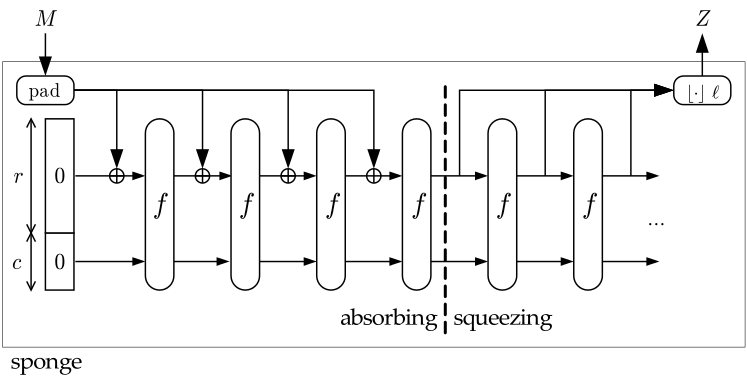
\includegraphics{images/esponja.png}
    \caption{Diagrama de uma função esponja}
    \label{fig:sponge}
\end{figure}

Os últimos $c$ bits não são diretamente afetados pela entrada $M$ e não são
produzidos como saída da função. A função esponja produz uma quantidade
indefinida de bits aleatórios.

\subsection{Função \Keccak}

A função de compressão \Keccak ($f$, não confundir com a compressão da esponja)
é uma função que tem como entrada um valor $S$ de $b$ \textit{bits}, de
$r + c = 1600$ bits no SHA-3. Esse valor $S$ é então dividido em uma matriz $A$
$5 \times 5$, onde cada célula contém 64 \textit{bits}. As posições dessa
matriz possuem índices $x$ (linha), $y$ (coluna) e $z$ (célula).

Uma vez criado esse estado interno, a função aplica 24 rodadas de processamento
$R_{i}$ que levam em consideração o resultado da rodada anterior e uma
constante $RC_{i}$

Cada uma das rodadas $R$ consiste na composição de cinco funções e pode ser
expressa pela seguinte função:

\begin{center}
    $R_{i} = \iota \circ \chi \circ \pi \circ \rho \circ \theta$
\end{center}

As funções possuem a seguinte fórmula:

\begin{itemize}
    \setlength\itemsep{1em}

    \item $\theta(M[x, y, z]) = M[x, y, z] \oplus \sum\limits_{y'=0}^{4}M[x-1, y', z] \oplus \sum\limits_{y'=0}^{4}M[x+1, y', z-1]$ \newline
        Este passo é uma função de substituição que utiliza bits de células
        adjacentes, cada \textit{bit} dependento de outros 11, o que provê boa
        difusão, que é importante para o efeito avalanche.

    \item $\rho(M[x, y, z]) = \begin{cases}
            M[x, y, z], \mbox{se } x=y=0 \\
            M[x, y, z - \frac{(t+1)(t+2)}{2}] \mid 0 \leq t < 24 \land \begin{pmatrix}0 & 1 \\ 2 & 3\end{pmatrix} \begin{pmatrix}0 \\ 1\end{pmatrix} = \begin{pmatrix}x \\ y\end{pmatrix}\mbox{ em } GF(5)
        \end{cases}$ \newline
        Função de espalhamento dos \textit{bits} de uma célula para auxiliar na
        difusão de forma mais rápida.

    \item $\pi(M[x, y]) = M[x', y'], \mid \begin{pmatrix}x \\ y\end{pmatrix}\begin{pmatrix}0 & 1 \\ 2 & 3\end{pmatrix} = \begin{pmatrix}x' \\ y'\end{pmatrix}$ \newline
        Outra função de espalhamento dos \textit{bits}, mas entre células
        diferentes.

    \item $\chi(M[x, y, z]) = M[x, y, z] \oplus (\neg{M}[x+1, y, z] \land M[x+2, y, z])$ \newline
        Esta função é uma substituição baseada no valor atual do bit e dos
        próximos 2 bits, tornando o \Keccak uma função não-linear,
        característica que os outros passos não provêm.

    \item $\iota(M[x, y, z]) = M[x, y, z] \oplus RC_{i}$, onde $RC_{i}$ é a
        constante da rodada citada acima e diferente para cada rodada $i$.

        Função de substituição baseada em uma tabela e que envolve uma
        constante que é diferente a cada passo da função aplicado.
\end{itemize}

\subsection{Parâmetros do SHA-3}

O SHA-3 define um algoritmo padrão para uso com parâmetros diferentes,
dependendo do nível de segurança e tamanho de \textit{bits} desejados na saída.
A tabela abaixo enumera os parâmetros normalmente utilizados com o SHA-3:

\begin{center}
    \renewcommand{\arraystretch}{1.2}
    \newcolumntype{M}[1]{>{\centering\arraybackslash}m{#1}}
    \begin{tabular}{ M{2.4cm} | M{2.4cm} | M{2.4cm} | M{2.4cm} | M{2.4cm} }
        Tamanho do valor de \textit{hash} & Tamanho do bloco $r$ & Capacidade $c$ & Resistência a colisão & Resistência a segunda pré-imagem \\ \hline
        224 & 1152 & 448 & $2^{112}$ & $2^{224}$ \\ \hline
        256 & 1088 & 512 & $2^{128}$ & $2^{256}$ \\ \hline
        384 & 832 & 768 & $2^{192}$ & $2^{384}$ \\ \hline
        512 & 576 & 1024 & $2^{256}$ & $2^{512}$
    \end{tabular}
\end{center}

Como visto nas seções anteriores, quanto maior o tamanho do bloco (ou
\textit{bitrate}), maior a vazão de \textit{bits}, porém menor a segurança do
SHA-3. Isto é evidente nos valores de resistência a colisão e à segunda
pré-imagem, que mostram que quanto menor é o \textit{bitrate}, maior é a
resistência. Observe também que, para os tamanhos de valor de \textit{hash} da
tabela acima, não há necessidade de se usar a fase de espremer a esponja do
algoritmo do SHA-3, pois é sempre menor que nestes casos.

\section{Questionário}

\let\oldsubsection\thesubsection%
\renewcommand{\thesubsection}{\thesection.\alph{subsection}}

\subsection{O que é e para que serve o \textit{state array}?}

O \textit{state array} do \Keccak é uma representação do estado do algoritmo e
uma matriz de três dimensões, de tamanho $5 \times 5 \times w$, onde $w$ é o
comprimento do bloco a ser cifrado. Na maioria das linguagens de programação,
é uma estrutura muito simples de ser representada, mas tem um uso bastante
complexo no \Keccak.

As partes bidimensionais dessa matriz são chamadas de \textit{plane} (plano),
\textit{slice} (fatia) e \textit{sheet} (folha), e as unidimensionais são
chamadas de \textit{row} (linha), \textit{column} (coluna) e \textit{lane}
(pista), conforme mostrado na figura~\ref{fig:statearray}. Um bit é indexado
por sua linha, coluna e pista.

\begin{figure}[ht]
    \centering
    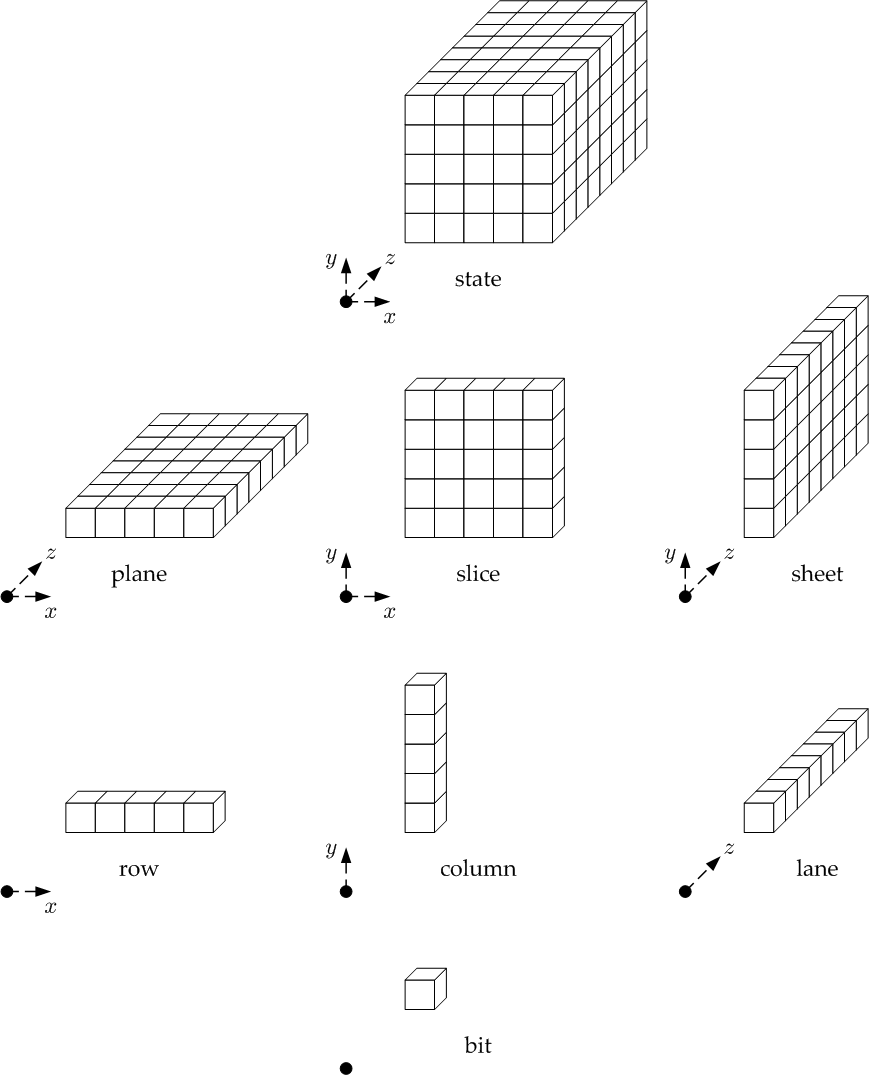
\includegraphics[width=0.7\textwidth]{images/statearray.png}
    \caption{Diagrama do \textit{state array}}
    \label{fig:statearray}
\end{figure}

O uso do \textit{state array} permite que as funções internas sejam definidas
em termos de posições nessa matriz de forma prática. O estado guarda valores
parciais do \textit{hash} e todas as funções internas recebem como parâmetro
o estado atual e retornam como saída o estado atualizado.

O primeiro valor do estado é gerado à partir da mensagem $S$ a ser cifrada, e o
resultado do \text{hash} é o estado após o último passo convertido novamente em
\textit{string}, passos estes que serão explicados nas próximas questões.

\subsection{Como é feita a conversão de \textit{strings} para
    \textit{state array}?}

Seja $S$ uma \textit{string} de $b$ \textit{bits} que representa o estado da
permutação \Keccak-$p[b, n_{r}]$. O \textit{state array} $A$ é definido da
seguinte forma no SHA-3, usando $b = 1600$ e $w = 64$:

Para toda tripla $(x, y, z)$ tal que $0 \leq x < 5$, $0 \leq y < 5$ e
$0 \leq z < w$,

\begin{center}
    $A[x, y, z] = S[w \cdot 5y + w \cdot x + z = S[w \cdot (5y+x) + z]$
\end{center}

Por exemplo, a posição $A[2, 1, 4]$ é obtida do \textit{bit}
$S[64 \cdot (5 \cdot 1 + 2) + 4] = S[772]$ da \textit{string} de entrada.

Usando essa fórmula, os \textit{bits} são mapeados sequencialmente por pista,
coluna e linha, ou seja, os primeiros 64 \textit{bits} serão mapeados na pista
da coluna 0 e linha 0, os próximos serão mapeados na pista da coluna 1 e linha
0, e assim sucessivamente.

É esta característica que gera o tamanho $b$ da string $S$, porque para cada
pista de $w$ \textit{bits}, existem $5 \cdot 5 = 25$ células pelo formato da
matriz, portanto $b = 25 \cdot w$.

\subsection{Como é feita a conversão de \textit{state array} para
    \textit{strings}?}

A conversão inversa, ou seja, de \textit{state array} para \textit{string}, é
feita de forma análoga, concatenando todas as pistas por coluna (gerando os
planos) e então por linha. Utilizando-se da mesma fórmula posicional,

\begin{center}
    $S[w \cdot (5y+x) + z] = A[x, y, z]$ \\
    ou \\
    $S[i] = A[\floor*{i \div (5w)}, \floor*{i \div w \pmod{w}}, i \pmod{w}]$
\end{center}

Primeiro se concatenam os $w$ \textit{bits} de uma pista:

$Lane(i, j) = A[i, j, 0] \concat A[i, j, 1] \concat \cdots \concat A[i, j, w-1]$

Onde $\concat$ denota concatenação de \textit{strings}, de forma que as pistas
da coluna $i = 0$, usando $w = 64$, sejam:

$\begin{array}{c}
    Lane(0, 0) = A[0, 0, 0] \concat A[0, 0, 1] \concat \cdots \concat A[0, 0, 63] \\
    Lane(1, 0) = A[1, 0, 0] \concat A[1, 0, 1] \concat \cdots \concat A[1, 0, 63] \\
    \vdots \\
    Lane(5, 0) = A[5, 0, 0] \concat A[5, 0, 1] \concat \cdots \concat A[5, 0, 63]
\end{array}$

E assim para todas as pistas. A \textit{string} que representa cada plano é a
concatenação de todas as pistas na sua coluna $j$:

$Plane(j) = Lane(0, j) \concat Lane(1, j) \concat \cdots \concat Lane(4, j)$

De forma que os planos de cada uma das colunas $0 \leq j < 5$ seja:

$\begin{array}{c}
    Plane(0) = Lane(0, 0) \concat Lane(1, 0) \concat \cdots \concat Lane(4, 0) \\
    Plane(1) = Lane(0, 1) \concat Lane(1, 1) \concat \cdots \concat Lane(4, 1) \\
    \vdots \\
    Plane(4) = Lane(0, 4) \concat Lane(1, 4) \concat \cdots \concat Lane(4, 4)
\end{array}$

A concatenação destes planos, então, gera a \textit{string} a partir do estado:

$S = Plane(0) \concat Plane(1) \concat \cdots \concat Plane(4)$

No resultado final, a concatenação de todos os \textit{bits} gera a seguinte
\textit{string}:

$S = A[0, 0, 0] \concat \cdots \concat A[0, 0, 63] \concat A[0, 1, 0] \concat \cdots \concat A[0, 4, 63] \concat A[1, 0, 0] \concat \cdots \concat A[4, 4, 63]$

\subsection{Explicar os cinco passos de mapeamento (\textit{step mappings})}

Cada rodada do SHA-3 é composta por cinco passos de mapeamento do \Keccak-$p$,
representados pelas funções $\iota$, $\chi$, $\pi$, $\rho$ e $\theta$, que
recebem como parâmetros posições de \textit{bits}, colunas e linhas e manipulam
o \textit{state array} da operação.

\subsubsection{Função \textit{theta} $\theta$}

A função \textit{theta} é definida pela seguinte fórmula:

$\theta(M[x, y, z]) = M[x, y, z] \oplus \sum\limits_{y'=0}^{4}M[x-1, y', z] \oplus \sum\limits_{y'=0}^{4}M[x+1, y', z-1]$

É uma função de substituição que utiliza os \textit{bits} de colunas adjacentes
e da mesma pista na qual está sendo aplicada. Para cada pista $A[x, y]$, cada
um dos $w$ \textit{bits} $z$ é logicamente somado com um somatório de uma
coluna da linha anterior e com um somatório de uma coluna da linha posterior,
como mostrado na figura~\ref{fig:theta}.

\begin{figure}[ht]
    \centering
    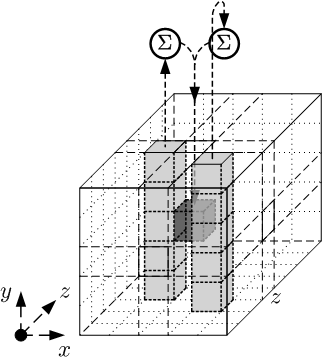
\includegraphics{images/theta.png}
    \caption{Visualização da função theta.}
    \label{fig:theta}
\end{figure}

Dessa forma, cada um dos \textit{bits} do \textit{state array} é afetado por
11 \textit{bits} do estado anterior, sendo 5 de cada coluna utilizada e o
próprio \textit{bit} em que a função foi aplicada. Isso cria um alto grau de
difusão dos efeitos de todas as funções no resultado.

A função \textit{theta} é a primeira porque mistura a parte interna do estado
(invisível para um atacante) com a parte externa, muito por causa do
funcionamento das funções esponja, portanto um atacante não pode acessar a
entrada das funções subsequentes apenas analisando a parte visível do estado.

\subsubsection{Função \textit{rho} $\rho$}

A função \textit{rho} é definida pela seguinte fórmula:

$\rho(M[x, y, z]) = \begin{cases}
    M[x, y, z], \mbox{se } x=y=0 \\
    M[x, y, z - \frac{(t+1)(t+2)}{2}] \mid 0 \leq t < 24 \land
    \begin{pmatrix}0 & 1 \\ 2 & 3\end{pmatrix}
    \begin{pmatrix}0 \\ 1\end{pmatrix} =
    \begin{pmatrix}x \\ y\end{pmatrix}
    \mbox{ em } GF(5)
\end{cases}$

É uma função de permutação que utiliza os \textit{bits} de uma pista $A[x, y]$.
No caso de $(x, y) = (0, 0)$, a função não altera os \textit{bits}, mas para
os outros casos, ela aplica um deslocamento circular dos \textit{bits} como um
embaralhamento dos mesmos, usando o valor $t$ para definir quantos bits será
deslocado, como mostrado na figura~\ref{fig:rho}.

\begin{figure}[ht]
    \centering
    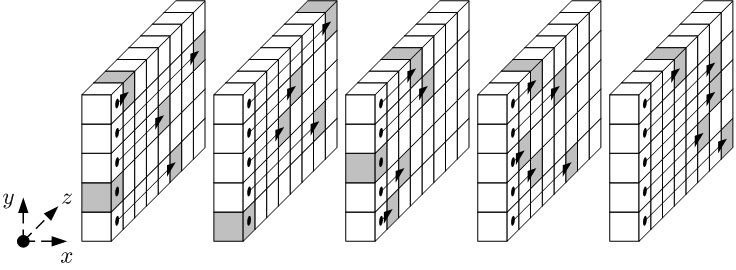
\includegraphics{images/rho.png}
    \caption{Visualização da função rho.}
    \label{fig:rho}
\end{figure}

Essa transformação gera a difusão entre os \textit{bits} de uma mesma pista,
acelerando os efeitos das funções em \textit{bits} próximos da \textit{string}
de entrada e do \textit{state array}, já que as outras funções criam difusão
entre linhas, colunas e pistas, mas não entre \textit{bits}.

\subsubsection{Função \textit{pi} $\pi$}

A função \textit{pi} é definida pela seguinte fórmula:

$\pi(M[x, y]) = M[x', y'] \mbox{ onde }
\begin{pmatrix}x' \\ y'\end{pmatrix} =
\begin{pmatrix}x \\ y\end{pmatrix}
\begin{pmatrix}0 & 1 \\ 2 & 3\end{pmatrix}$

É uma função de permutação que utiliza as pistas. Assim como \textit{theta},
\textit{pi} faz um deslocamento circular usando uma fórmula semelhante, como
mostrado na figura~\ref{fig:pi}.

\begin{figure}[ht]
    \centering
    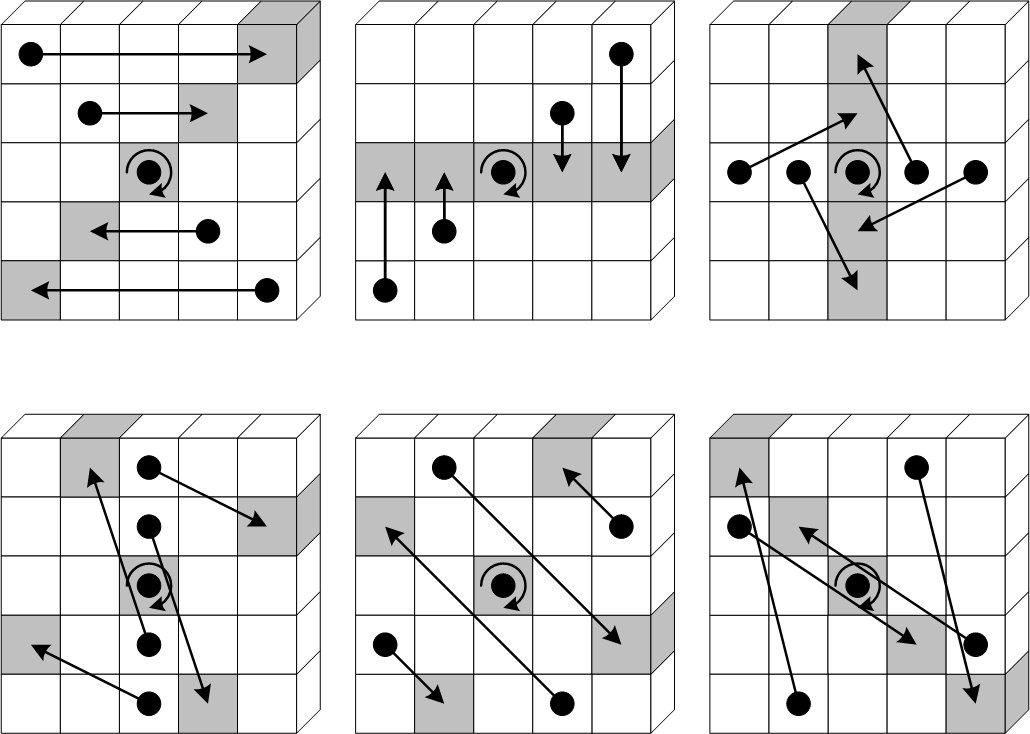
\includegraphics[width=0.7\textwidth]{images/pi.png}
    \caption{Visualização da função pi.}
    \label{fig:pi}
\end{figure}

Essa transformação gera a difusão entre diferentes pistas.

\subsubsection{Função \textit{chi} $\chi$}

A função \textit{chi} é definida pela seguinte fórmula:

$\chi(M[x, y, z]) = M[x, y, z] \oplus (\neg{M}[x+1, y, z] \land M[x+2, y, z])$

É uma função de substituição que utiliza os \textit{bits} posteriores ao
\textit{bit} sendo aplicado, sendo o passo não-linear que torna a função
\Keccak uma função irreversível, ou seja, impede a obtenção da pré-imagem a
partir do \textit{hash}. O passo \textit{chi} é mais facilmente visualizado se
usando um circuito digital, como mostrado na figura~\ref{fig:chi}.

\begin{figure}[ht]
    \centering
    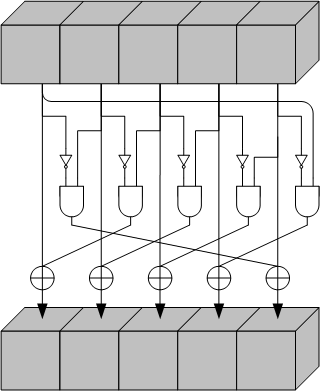
\includegraphics{images/chi.png}
    \caption{Visualização da função chi.}
    \label{fig:chi}
\end{figure}

Sua definição possui propriedades algébricas que garantem que a saída não
possui correlação direta com a entrada em termos de paridade, ou seja, não é
possível concluir nada sobre a entrada analisando a quantidade de \textit{bits}
em 0 ou 1 da saída.

\subsubsection{Função \textit{iota} $\iota$}

A função \textit{iota} é definida pela seguinte fórmula:

$\iota(M[x, y]) = M[x, y] \oplus RC_{i}$

É uma função de substituição baseada em um valor tabelado e diferente para cada
rodada do SHA-3, e é gerado a partir de uma fórmula que utiliza um gerador de
deslocamento linear realimentado (LFSR, na sigla em inglês) em $GF(2)$:

$RC_{i}[2^{j}-1] = (x^{j+7i} \pmod{x^8 + x^6 + x^5 + x^4 + 1}) \pmod{x} \mbox{ para } 0 \leq j \leq \log w$

Dessa forma, não existe relação de simetria entre as diferentes rodadas, porque
sem este passo, todas as rodadas teriam a mesma fórmula e poderiam ser
simplificadas para permitir ataques.

A função \textit{iota} é somente aplicada na primeira linha e coluna, ou seja,
os parâmetros $x$ e $y$ são sempre 0, e seu efeito é difundido para as outras
linhas e colunas através dos passos \textit{theta} e \textit{chi}.

\subsection{Explicar a permutação \Keccak-$p[b,n_r]$}

Uma função \Keccak-$p[b, n_r]$ é uma generalização das funções de substituição
e permutação \Keccak que podem ser usadas pelo SHA-3 e recebe como parâmetros o
comprimento da \textit{string} $S$, que define o tamanho do
\textit{state array}, e o número de rodadas na fase de absorção.

Cada uma das rodadas $R_{i}$ de \Keccak-$p$ consiste na aplicação dos cinco
passos de transformação, vistos na seção anterior:

\begin{center}
    $R_{i} = \iota \circ \chi \circ \pi \circ \rho \circ \theta$
\end{center}

O \textit{state array} na rodada $i$, denominado $S_{i}$, é encontrado pela
seguinte composição de funções:

\begin{center}
    $S_{i} = \iota(\chi(\pi(\rho(\theta(S_{i-1}))), i)$
\end{center}

Onde $j \geq 2l + 12 - n_r$, sendo $l = \log w$, e $i < 2l + 12$. Essa
definição genérica nos permite gerar versões do \Keccak para diferentes
tamanhos de palavras $w$, desde que $w = 2^{k}$. É conveniente utilizar $32$ ou
$64$ por ser o tamanho de uma palavra em processadores modernos, e o FIPS 202
define os seguintes parâmetros por padrão:

$\begin{array}{l}
    b \in \{25, 50, 100, 200, 400, 800, 1600\} \\
    n_{r} = 2l + 12, \mbox{ onde } l \in \mathbb{Z}
\end{array}$

\subsection{Descrever o \textit{framework} \textit{sponge construction}}

Funções esponja são uma classe de funções que recebem uma entrada de tamanho
finito qualquer e produzem uma saída com outro tamanho qualquer desejado, sendo
definidas por três parâmetros: um estado $S$, que contém $b$ bits; uma função
$f$ que permuta ou transforma o estado $S$; e uma função de \textit{padding}
$P$~\cite{noekeon:2011}.

Na inicialização, a função $P$ é aplicada na entrada $M$ e dividida em blocos
de $r$ bits. Os $b$ bits do estado $S$ são zerados. A construção da esponja se
dá em duas fases, chamadas de absorção e compressão.

O tamanho $r$ também é chamado de \textit{bitrate}, porque representa a
quantidade de bits da entrada que são consumidos em cada iteração da função
esponja, e o tamanho $c = |S| - r$ é chamado de capacidade, e representa o
nível de segurança atingido pela variante da função - SHA-3, $r + c = b$.

Na fase de absorção, cada bloco $P$ de $r$ bits é combinado com os primeiros
$r$ bits, com os restantes $c$ bits preenchidos com zero, do estado $S$ com
\texttt{xor} e é aplicada a função $f$ no resultado, ou seja,
$S_{i} = f(S_{i-1} \oplus P_{i} \concat 0^{c})$. Ao final de todas as
iterações, ou seja, após a mensagem $M$ ser completamente consumida pela
absorção da esponja, a saída da função $f$ será o \textit{hash} gerado. Na fase
de compressão, os primeiros $r$ bits do estado $S$ são retornados, e caso mais
bits sejam desejados, se aplica novamente a função $f$ em $S$ para transformar
o estado.

\subsection{Explique a família de funções esponja \Keccak}

\subsection{Explique a especificação da função SHA-3}

A definição do SHA-3 publicada pelo NIST prevê dois tipos de função baseadas no
\Keccak, funções de \textit{hash} criptográficas e funções de saída extendida
(XOF), também chamadas de SHAKE.

\begin{enumerate}[label=\roman*.]
    \setlength\itemsep{1em}

    \item Funções de \textit{hash} SHA-3

        As funções de \textit{hash} podem ser definidas genericamente para um
        tamanho do \textit{hash} gerado $d$ e mensagem $M$ com a seguinte
        fórmula:

        $SHA-3(d, M) =$ \Keccak-$p[2d](M \concat 01, d)$ \newline

        Observando que os bits $01$ são concatenados à mensagem $M$ antes da
        execução a função. O NIST definiu os tamanhos
        $d \in \{224, 256, 384, 512\}$ para o SHA-3, existindo portanto
        SHA3-224, SHA3-256, SHA3-384 e SHA3-512.

    \item Funções de saída extendida
\end{enumerate}

\subsection{Apresente a análise de segurança}

\subsection{Exemplos}

\let\thesubsection\oldsubsection%

\section{Implementação}

O algoritmo foi implementado em \textbf{C++11} em uma classe \textit{template},
que pode ser configurada para diferentes capacidades e tamanhos de saída em
tempo de compilação. Dessa forma, é possível declarar diferentes instâncias de
\Keccak, como será mostrado após o código. Além disso, se faz necessária uma
função de rotação lógica de inteiros, denominada \texttt{rotl}:

\lstinputlisting[language={[11]C++},firstline=4,lastline=182]{Keccak.h}

As cinco funções de transformação $\theta$, $\rho$, $\pi$, $\chi$ e $\iota$
foram implementadas como métodos que recebem o estado atual e retornam o estado
transformado, com a última ($\iota$) também recebendo o gerador das constantes
de cada rodada.

Além disso, a classe funciona como uma máquina de estados, que está
``absorvendo'' (\texttt{ABSORBING}) ou ``espremendo'' (\texttt{SQUEEZING}),
necessariamente nesta ordem. Um objeto \texttt{Keccak} inicializa com a fase
\texttt{ABSORBING} e muda para a fase \texttt{SQUEEZING} quando a função de
padding é executada.

Além disso, uma função auxiliar \texttt{squeeze\_more} gera mais saída, para
uso no caso das funções de saída extendida, transformando o estado conforme
necessário e armazenando no \textit{stream} \texttt{output}, que a função que
retorna o hash consulta.

O atributo \texttt{npos} possui dois significados: na fase de absorção,
representa quantos \textit{bytes} já foram inseridos no estado; após, informa
quantos \textit{bytes} estão disponíveis em \textit{output}, uma vez que
\textit{streams} não possuem um contador de quantidade de dados disponível.

Uma classe \texttt{SHA3} foi declarada contendo uma única função \texttt{hash},
que automaticamente cria uma instância de \texttt{Keccak}, insere a mensagem
no estado, aplica o padding e retorna o \textit{hash} no tamanho desejado,
usando como padrão a proporção indicada pelo \textbf{FIPS 202}.

Uma classe \texttt{SHAKE} foi declarada contendo as funções \texttt{update},
\texttt{finalize} e \texttt{digest}, que inserem mais valores no estado, trocam
o estado da função e extraem uma quantidade variável de \textit{bytes},
respectivamente com assinaturas baseadas em outras bibliotecas do gênero, como
o \textbf{OpenSSL}.

Dessa forma, é trivial declarar funções com os parâmetros definidos pelo NIST:

\lstinputlisting[language={[11]C++},firstline=184,lastline=219]{Keccak.h}

É importante ressaltar que a todas as funções podem ser aplicadas em uma
\textit{lane} em vez de aplicadas \textit{bit} a \textit{bit}, por isso é mais
eficiente trabalhar com inteiros (neste caso, \texttt{uint64\_t}) do que com
\textit{bitsets}. Está disponível no documento do FIPS 202~\cite{fips:2015} e
na referência do \Keccak~\cite{keccak:2011} o pseudocódigo que gera os mesmos
resultados. O código acima completo está disponível no
GitHub~\cite{althoff:2016}.


\bibliographystyle{sbc/sbc}
\bibliography{sha-3}

\end{document}
